\section{Implementacja}
W tym rozdziale opisane zostały najistotniejsze elementy aplikacji: wybrane funkcje, ich opisy oraz wszystkie dostępne widoki z podziałem na użytkownika i administratora. 
Przedstawione zostały 3 moduły: moduł map, moduł zgłaszania zagrożeń oraz moduł powiadomień. Pierwszy z nich prezentuje metody odpowiedzialne za wygląd mapy oraz nawigację po niej. Moduł zgłaszania zagrożeń zawiera funkcje, które zapisują informacje o niebezpieczeństwach na szlakach, natomiast moduł powiadomień odpowiedzialny jest za ostrzeganie użytkowników o czyhających zagrożeniach.
\subsection{Moduł map}
Podrozdział został poświęcony na dokładne przyjrzenie w jaki sposób działają funkcje, które umożliwiają poruszanie się po górach oraz wpływają na wygląd mapy. Każda z nich sprawia, iż użytkownik ma możliwość pokonania wybranej trasy, a naniesione na mapę szlaki pozwalają mu zaplanować wędrówkę w każdym momencie. Poniżej przedstawione zostały wybrane funkcje składające się na implementację rysowania szlaków, wyznaczenia trasy, zapisu lokalnego plików oraz obsługi ikon ze schroniskami, szczytami i stawami.
\\ 
\\
\textbf{Implementacja rysowania szlaków na mapie} \\
\indent Fragment kodu, zaprezentowany na listingu \ref{lst:rysowanie} odczytuje dane z pliku KML i na ich podstawie rysuje szlaki na mapie. Za pomocą FileInputStream zostaje stworzony strumień wejściowy do odczytania pliku, który potrzebny jest do utworzenia warstwy KML. Następnie jest ona dodawana do mapy i rozpoczyna się iterowanie po kontenerach. Pętla odczytująca obiekty KmlPlacemark, pobiera ich nazwę i na jej podstawie określa kolor szlaku. \\W kolejnym kroku zostają zdefiniowane opcje linii, czyli wybrany kolor oraz szerokość. Jeżeli geometria danego znacznika jest linią (KmlLineString), tworzona jest lista, przechowująca współrzędne szlaku, które następnie dodane są do wcześniej zdefiniowanej linii. Na koniec, utworzona trasa zostanie narysowana na mapie, dzięki czemu użytkownik widzi wszystkie szlaki Tatr. Efekt ten widoczny jest na rys.\ref{widok:map}.\\

\noindent
\begin{minipage}{\linewidth}
    \captionof{listing}{Funkcja odpowiedzialna za rysowanie szlaków na mapie}
    \label{lst:rysowanie}
    \centering
    \fbox{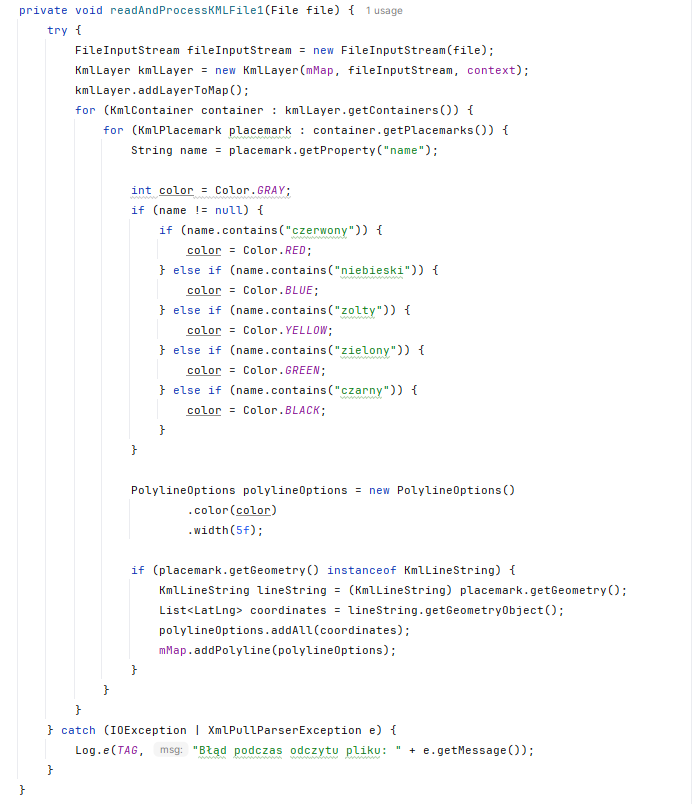
\includegraphics[width=0.6\linewidth]{img/kod/rysowanie-szlakow.png}}
\end{minipage}\\

\\
\noindent \textbf{Implementacja lokalnego zapisu plików} \\ 
\indent Funkcja przedstawiona na rys. \ref{lst:pobierz} odpowiada za kontrolę pobierania plików z serwera (Firebase Storage) i jest wywołana po każdym uruchomieniu aplikacji. Pliki zawierają informacje o szlakach oraz punktach, w których znajdują się schroniska, szczyty oraz stawy. Na początku funkcja tworzy obiekt reprezentujący ścieżkę do katalogu w pamięci i sprawdza, czy istnieje on fizycznie, jeśli nie, tworzy go. Następnie ustala pełną ścieżkę do lokalnego pliku \\i również sprawdza czy istnieje. Dalszy fragment kodu porównuje jego rozmiar z rozmiarem wersji na serwerze, aby określić, czy pobranie nowej wersji jest konieczne. Jeśli lokalny plik różni się zostaje on pobierany ponownie. Działanie funkcji sprawia, iż użytkownik ma zawsze aktualne dane zapisane na swoim urządzeniu. 
\\

\noindent
\begin{minipage}{\linewidth}
    \captionof{listing}{Funkcja odpowiedzialna za lokalny zapis plików.}
    \label{lst:pobierz}
    \centering
    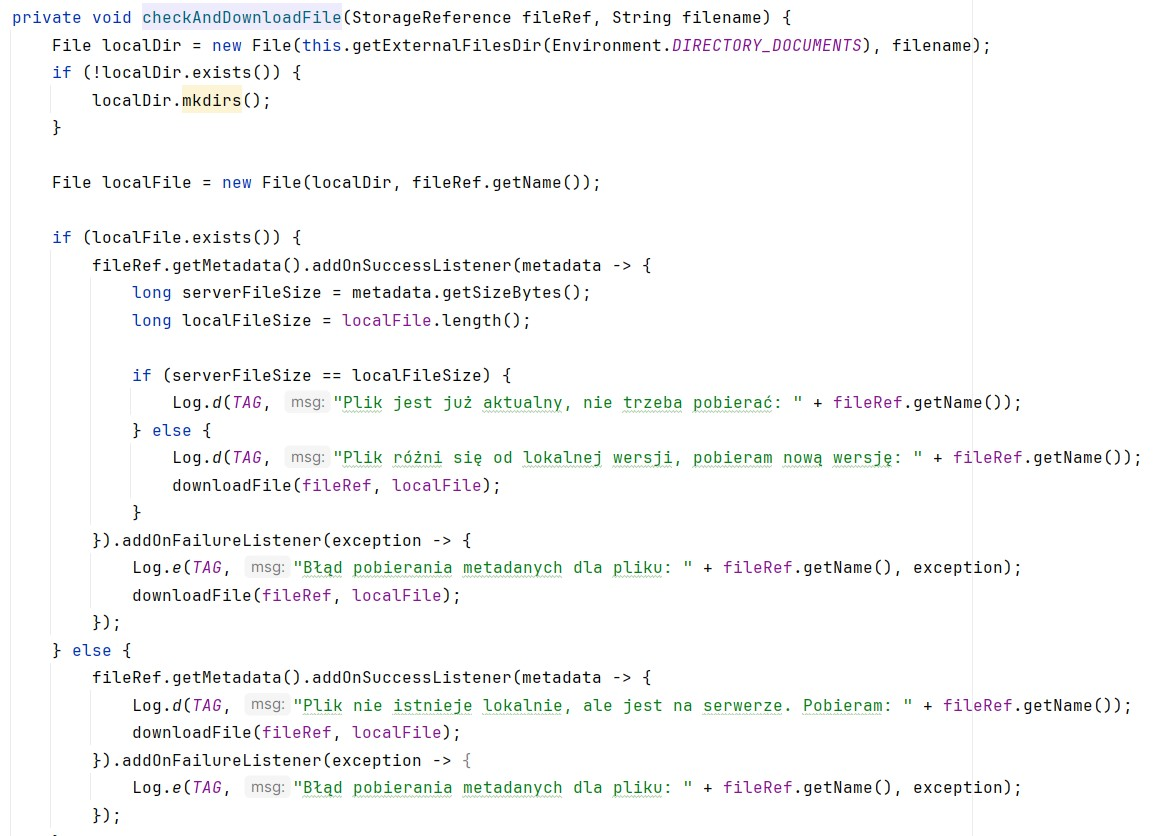
\includegraphics[width=0.6\linewidth]{img/kod/imp-ckeckandadd.jpg}
\end{minipage}\\

\\

\noindent
\textbf{Implementacja ikon ze schroniskami, szczytami oraz stawami} \\ 
\indent Fragment kodu przestawiony na listingu \ref{lst:schron} odpowiada za odczyt danych z pliku i utworzenie listy markerów. Użycie XmlPullParser umożliwia analizę pliku i pobranie danych potrzebnych do stworzenia markera. Po jego konfiguracji, następuje iterowanie po pliku, aż do osiągnięcia końca dokumentu. Podczas iteracji funkcja odczytuje dane z konkretnych tagów, kolejno nazwę z \verb|<name>|, opis \verb|<description>| oraz współrzędne \verb|<coordinates>|. Po napotkaniu na tag zamykający \verb|<Placemark>| i sprawdzeniu czy lokalizacja jest poprawna, zostaje utworzony marker z ikoną pokazaną jako parametr funkcji. Następnie jest on dodany do listy, która umożliwia kontrolę widoczności markerów. \\

\noindent
\begin{minipage}{\linewidth}
    \captionof{listing}{Funkcja odpowiedzialna za wyświetlanie na mapie ikon schronisk, szczytów oraz stawów.}
    \label{lst:schron}
    \centering
    \fbox{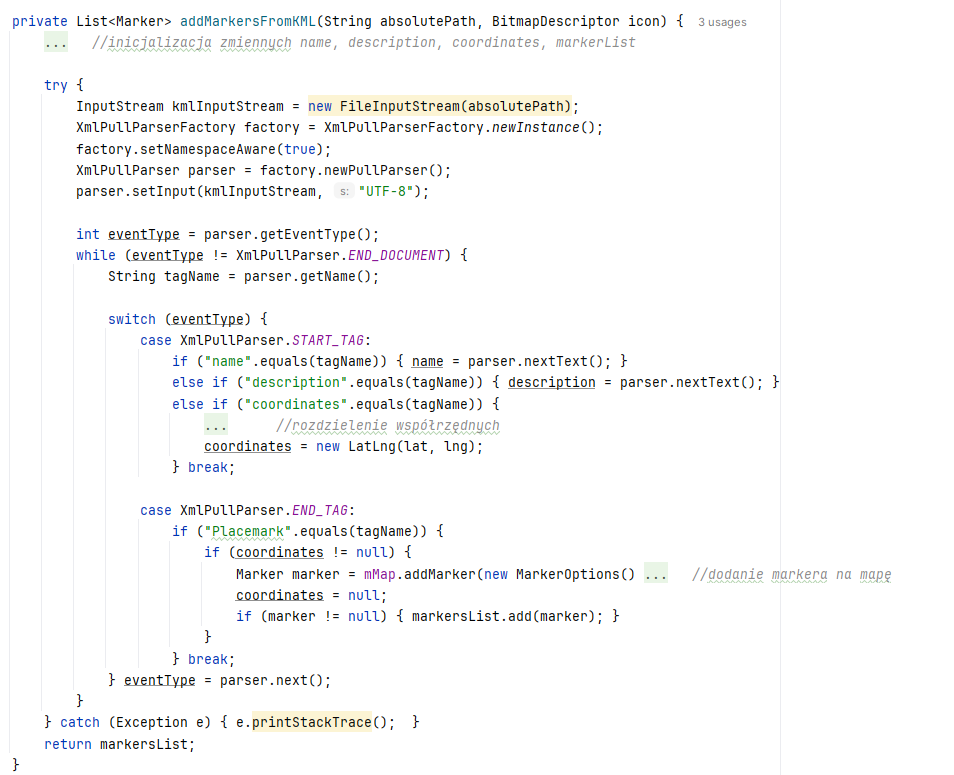
\includegraphics[width=0.6\linewidth]{img/kod/schroniska.png}}
\end{minipage}\\


\textbf{Implementacja wyznaczenia trasy}\\
\indent Za wyznaczanie trasy odpowiedzialnych jest kilka funkcji. Jedna z nich została przedstawiona na listingu \ref{lst:trasa} i służy do utworzenia adresu URL, który definiuje trasę. Początek kodu sprawdza, czy dane trasy są puste, jeśli tak, zostanie rzucony wyjątek z informacją o tym, jeśli nie, zostaje wykonany dalszy kod. Określone zostają informacje o wyznaczonej trasie, t.j. początek i koniec oraz tryb pieszy, a także klucz API Google Maps, potrzebny do poprawnego stworzenia adresu URL. Funkcja \verb|encodeLatLng()| konwertuje współrzędne, tak aby pasowały do jego formatu. Kolejnym krokiem jest sprawdzenie, czy trasa posiada przystanki, jeśli tak, ich współrzędne są pobieranie i dodane do ciągu znaków. Na koniec, wszystkie parametry połączone zostają w jeden ciąg tekstowy, którym jest gotowy adres URL. Link zawiera wynik trasy w formacie JSON, który jest odbierany i przetwarzany przez kolejne funkcje, które nie zostały opisane ze względu na ich ilość. Po wykonaniu ich wszystkich, można \\z odczytać szczegółowe dane drogi, wybranej przez użytkownika. \\

\noindent
\begin{minipage}{\linewidth}
    \captionof{listing}{Funkcja odpowiedzialna za wyznaczanie trasy}
    \label{lst:trasa}
    \centering
    \fbox{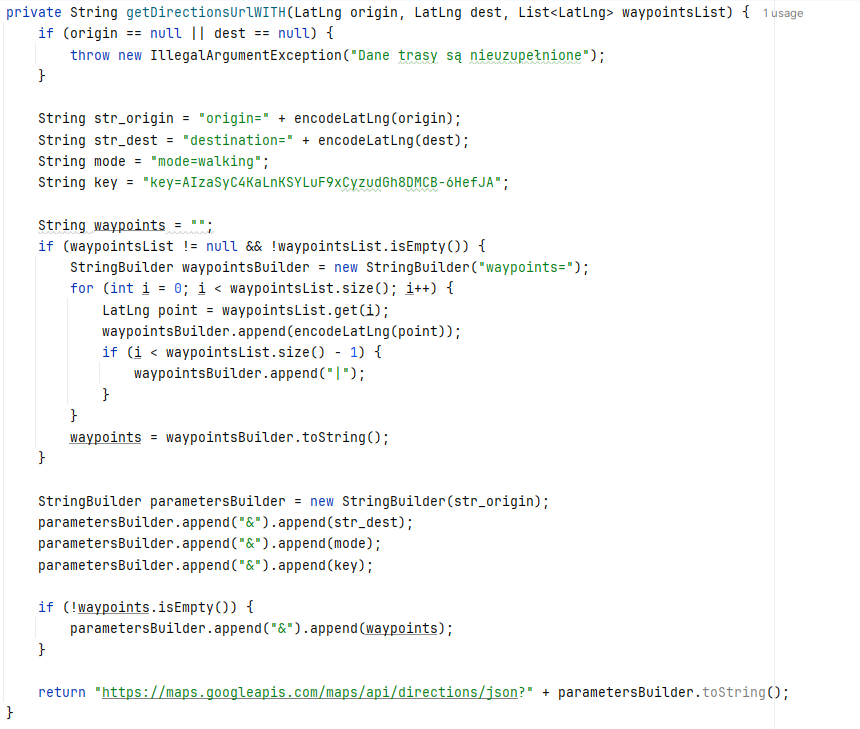
\includegraphics[width=0.6\linewidth]{img/kod/trasa.png}}
\end{minipage}
\\

Funkcja, przedstawiona na listingu \ref{lst:rystras} rysuje wyznaczoną trasę z przetworzonego wyniku, uzyskanego z adresu URL. Przed pobraniem współrzędnych linii, mapa jest czyszczona z innych tras. Następnie tworzonych jest kilka obiektów: lista punktów nowej ścieżki, zbiór z unikalnymi punktami, który zapobiega powielaniu takich samych współrzędnych oraz linia, reprezentująca nową trasę. Podczas iteracji, pobierane są współrzędne każdego punktu na ścieżce i na ich podstawie utworzony zostaje obiekt LatLng. Jeśli dodanie jego do zbioru \verb|uniquePoints| przejdzie pomyślnie, zostanie on dodany do listy z punktami trasy. W kolejnym kroku wyznaczona droga, zostanie zdefiniowana o te współrzędne, kolor oraz szerokość. Następnie funkcja rysuje ją na mapie i aktualizuje listę jej punktów. Na koniec, kamera zostanie ustawiona na pierwszy punkt trasy z określonym przybliżeniem, dzięki czemu użytkownik może rozpocząć wędrówkę po swojej ścieżce.\\

\noindent
\setlength{\fboxrule}{0.5pt}
\begin{figure}[H]
    \centering
    \fbox{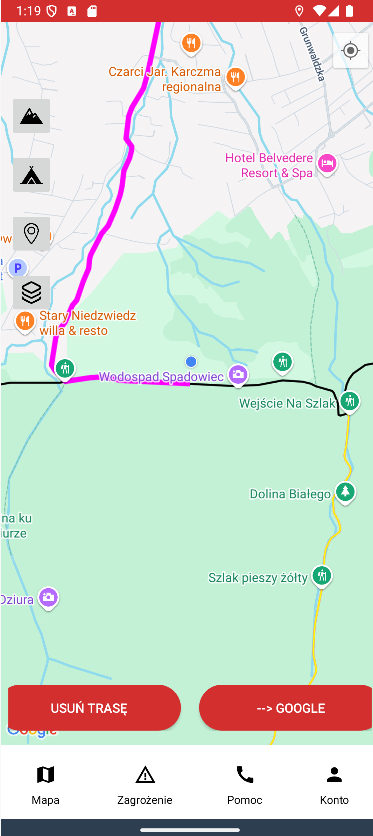
\includegraphics[scale=0.6]{img/imp/widok-trasa.png}}
    \caption{Pokazanie efektu po zatwierdzeniu wybranej przez użytkownika trasy.}
    \label{widok:zatwierdztrase}
\end{figure}
\\

\noindent
\setlength{\fboxrule}{0.5pt}
\begin{minipage}{\linewidth}
    \captionof{listing}{Funkcja odpowiedzialna za rysowanie szlaków na mapie}
    \label{lst:rystras}
    \centering
    \fbox{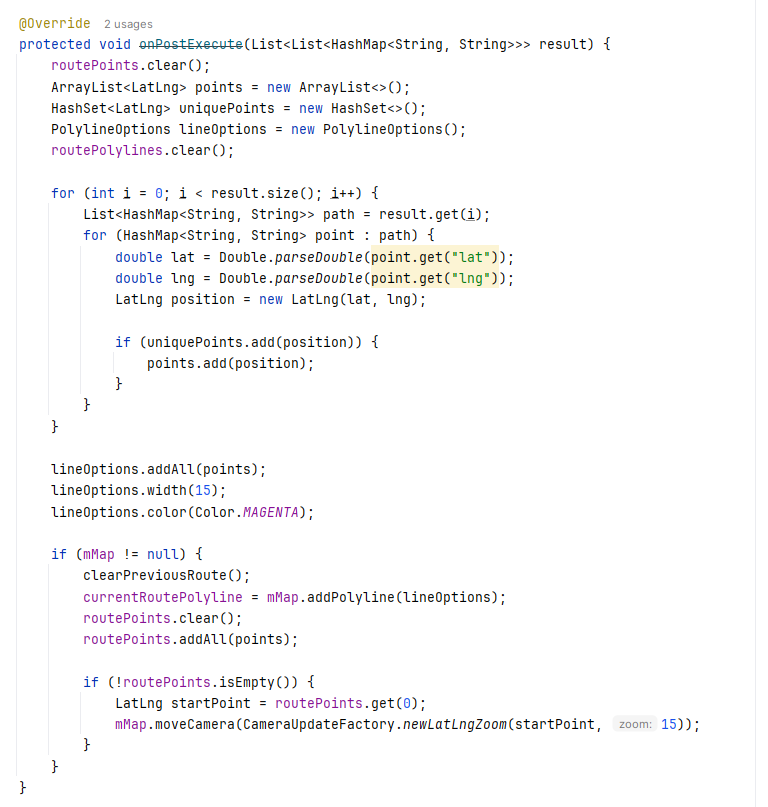
\includegraphics[width=0.6\linewidth]{img/kod/rys-tras.png}}
\end{minipage}
\\

\subsection{Moduł zgłoszeń}
Przy procesie obsługi zgłoszeń uczestniczy zarówno użytkownik jak i administrator. Pierwszy z nich zgłasza zagrożenie, podając wszystkie niezbędne informacje o niebezpieczeństwie. Drugi natomiast decyduje, czy dane zgłoszenie jest pomocne dla innych użytkowników.  Poniżej zostały przedstawione najważniejsze funkcje składające się na implementację zapisu zgłoszeń do bazy Firebase oraz akceptację zgłoszeń.
\\

\noindent
\textbf{Implementacja zapisu zgłoszeń do bazy (Firebase)} \\ 
\indent Fragment kod, pokazany na rys. \ref{lst:danger} odpowiada za zapis zgłoszenia do bazy. Na początku sprawdzone zostaje połączenie z internetem, jeśli go nie ma, dane zostają zapisane lokalnie na urządzeniu, za co odpowiedzialna jest funkcja \verb|saveDangerLocally()|. W przypadku, gdy użytkownik ma włączony internet i GPS, zostaje zapisana jego lokalizacja oraz możliwe jest pobranie jego nazwy oraz email. Na podstawie danych o zalogowanym zostaje utworzony obiekt  \verb|Map<String, Object>|, który jest potrzebny do poprawnego zapisu zgłoszenia. Następnie dane przekazane w parametrze funkcji zostają dodane do obiektu “danger”, który zawiera informacje o zagrożeniu. \\W kolejnym kroku zostają one zapisane do bazy. W przypadku niepowodzenia zostaje wyświetlony komunikat o błędzie. \\

\noindent
\setlength{\fboxrule}{0.5pt}
\begin{minipage}{\linewidth}
    \captionof{listing}{Funkcja odpowiedzialna za zapis zgłoszeń do bazy.}
    \label{lst:danger}
    \centering
    \fbox{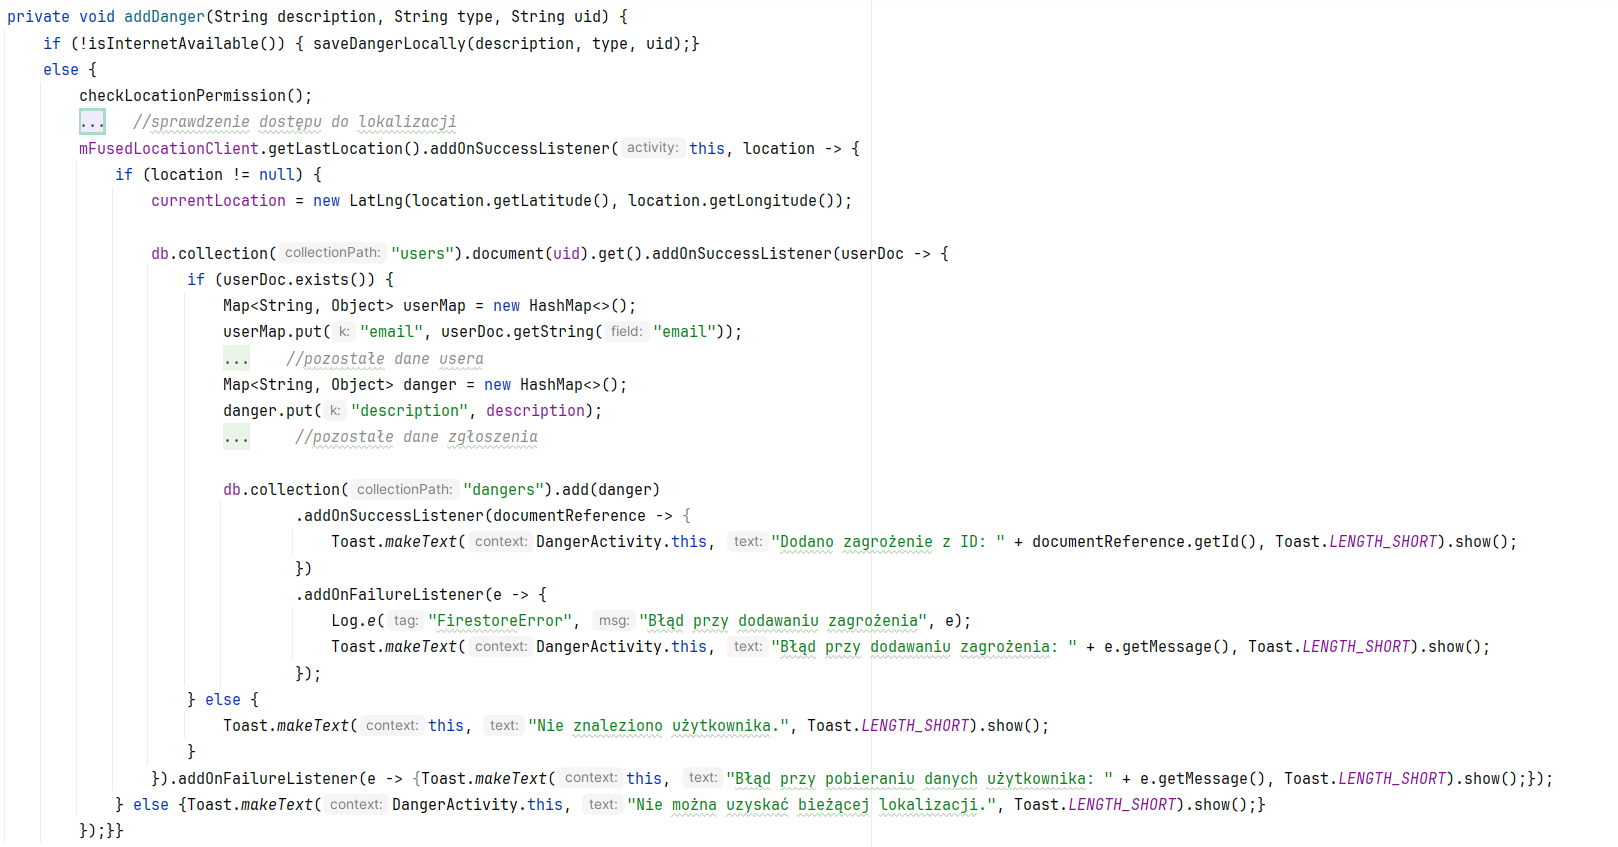
\includegraphics[width=0.6\linewidth]{img/kod/imp-adddanger.png}}
\end{minipage}
\\

\noindent
\textbf{Implementacja akceptacji zgłoszeń} \\ 
\indent Funkcja, pokazana na rys. \ref{lst:accepted} odpowiada za aktualizację danych zgłoszenia, a dokładniej ustawienie wartości pola “accepted” na “true”. Na podstawie identyfikatora dokumentu, przekazanego w parametrze funkcji, wiadome jest, które zgłoszenie należy zaktualizować. Skutki działania tego fragmentu kodu są wykorzystane w innych funkcjach aplikacji, np. \verb|getAccpetDangersLocations()|, opisanej poniżej.

\noindent
\setlength{\fboxrule}{0.5pt}
\begin{minipage}{\linewidth}
    \captionof{listing}{Funkcja odpowiedzialna za akceptację zgłoszeń.}
    \label{lst:accepted}
    \centering
    \fbox{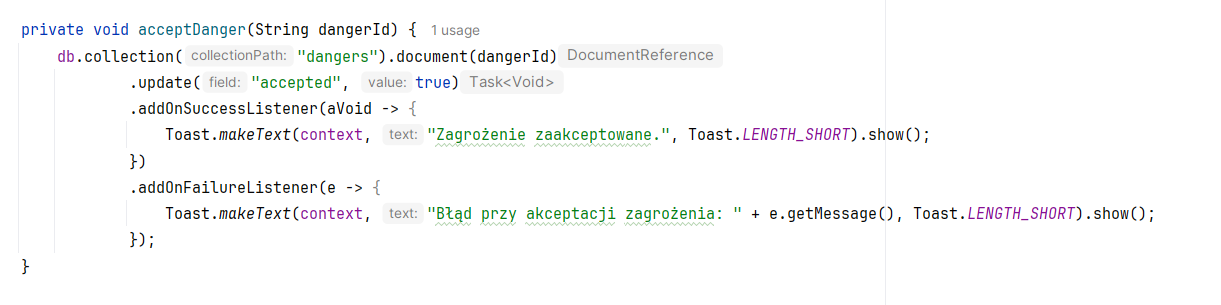
\includegraphics[width=0.6\linewidth]{img/kod/imp-acceptdanger.png}}
\end{minipage}
\\

Funkcja przedstawiona na rys. \ref{lst:getaccepted} służy do pobierania lokalizacji zgłoszeń zagrożeń, które zostały zaakceptowane. Na początku dane są filtrowane, tzn. sprawdzane jest czy dane zgłoszenie w polu dokumentu “accepted” ma wartość “true”. W przypadku niepowodzenia podczas pobierania danych z bazy, zostaje wyświetlony komunikat, informujący o takiej sytuacji. Jeśli pobieranie danych zakończy się powodzeniem i wyniki filtrowania nie są puste, następuje iteracja przez każdy dokument. W kolejnym kroku jest sprawdzane czy posiada on pole “location”, jeśli tak, dane zostają pobrane i zapisane do \verb|Map<String, Object>|. Kluczem stworzonej mapy jest “latitude” lub “longitude”, a wartością współrzędne. Następnie, dane te są łączone w jeden obiekt LatLng, reprezentujący miejsce, w którym zostało wykonane zgłoszenie. Na koniec, współrzędne są dodawane do listy, przechowującej lokalizacje zaakceptowanych zgłoszeń. Po sprawdzeniu czy nie jest ona pusta zostaje wywołana funkcja \verb|updateMapWithAcceptedDangers()|, przedstawiona na rys. \ref{lst:markeraccepted}. Odpowiada ona za ustawienie markerów na mapie w miejscu, wystąpienia zagrożenia. \\

\noindent
\setlength{\fboxrule}{0.5pt}
\begin{minipage}{\linewidth}
    \captionof{listing}{Funkcja odpowiedzialna za pobranie lokalizacji zgłoszeń.}
    \label{lst:getaccepted}
    \centering
    \fbox{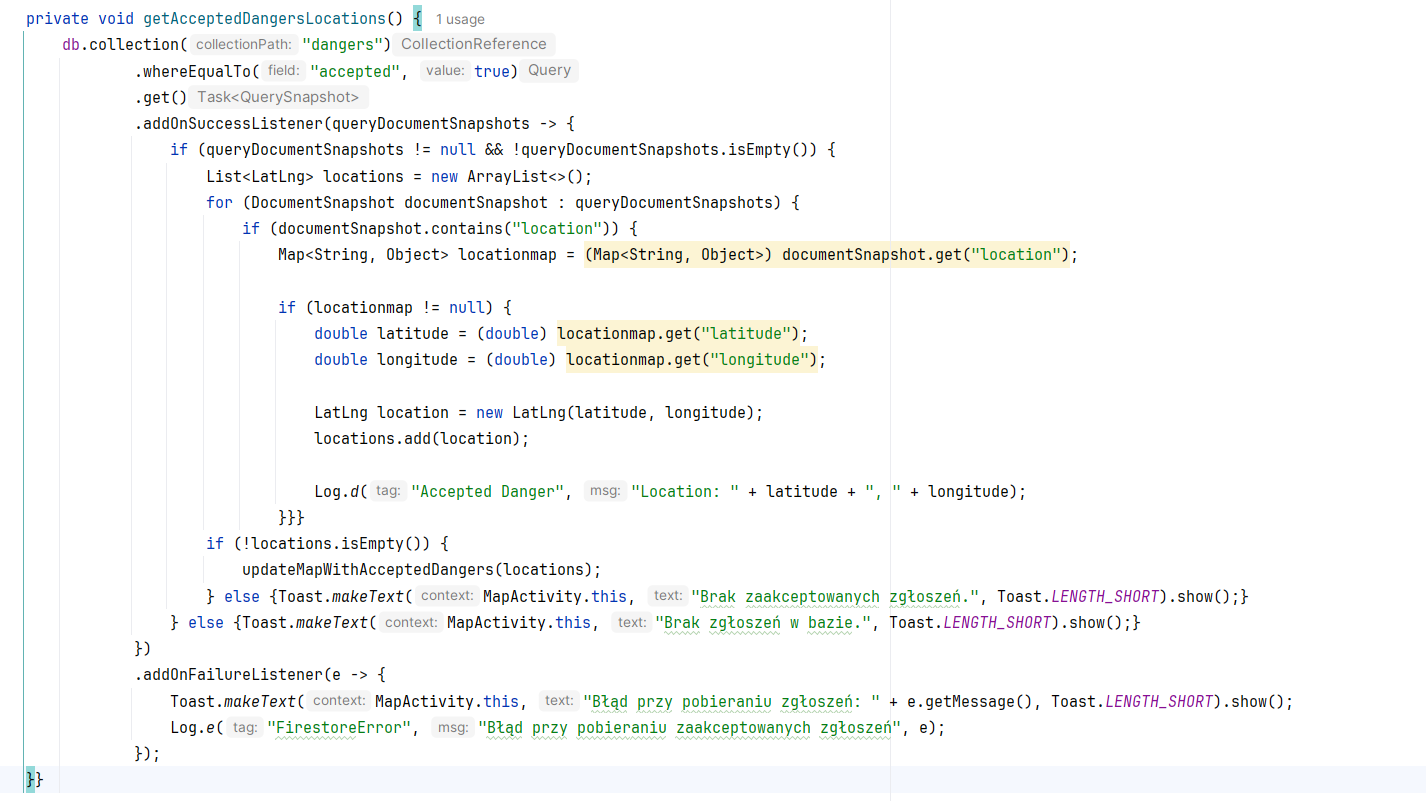
\includegraphics[width=0.6\linewidth]{img/kod/imp-getacceptedloc.png}}
\end{minipage}
\\
\\
\\
\noindent
\setlength{\fboxrule}{0.5pt}
\begin{minipage}{\linewidth}
    \captionof{listing}{Funkcja odpowiedzialna za ustawienie markerów z zagrożeniami na mapie.}
    \label{lst:markeraccepted}
    \centering
    \fbox{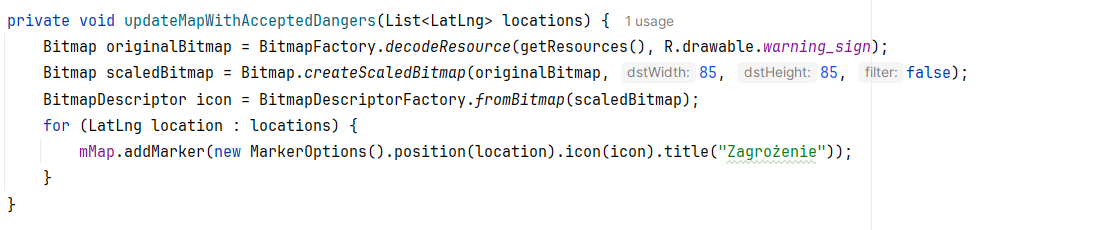
\includegraphics[width=0.6\linewidth]{img/kod/imp-updatemap.png}}
\end{minipage}


\noindent
\setlength{\fboxrule}{0.5pt}
\begin{figure}[H]
    \centering
    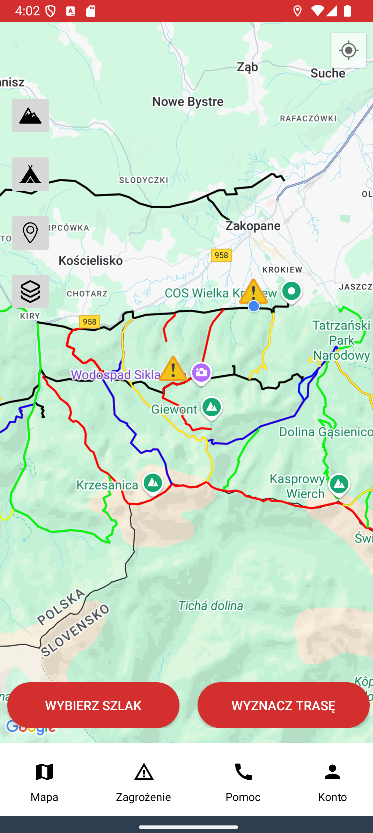
\includegraphics[scale=0.6]{img/imp/test-accpeted.png}
    \caption{Zaktualizowana mapa po akceptacji zgłoszeń przez administratora.}
    \label{widok:markeraccepted1}
\end{figure}
\\
\subsection{Moduł logowania i rejestracji}
Logowanie i rejestracja pozwala na łatwe zidentyfikowanie użytkownika aplikacji, a także pozwala na śledzenie jego aktywności celem stworzenia raportów czy wykresów. Pozwala też na ustalenie, który użytkownik wysłał zgłoszenie o zagrożeniu. Poniżej przedstawione są funkcje niezbędne do implementacji logowania oraz rejestracji nowych użytkowników \\w systemie.
\\

\noindent
\textbf{Implementacja rejestracji}\\
\indent Rejestracja w tej aplikacji opiera się na adresie email oraz haśle i wybraniu nazwy użytkownika, Wszystkie te dane muszą być podane, aby rejestracja przebiegła pomyślnie. Do zabiegu rejestracji wykorzystywany jest moduł Firebase Authentication ułatwiający autoryzację użytkowników. Cała rejestracja kryje się pod przyciskiem "Zarejestruj" na widoku rejestracji użytkownika.\\
\noindent
\setlength{\fboxrule}{0.5pt}
\begin{minipage}{\linewidth}
    \captionof{listing}{Rejestracja użytkownika w "słuchaczu" przycisku "Zarejestruj".}
    \label{lst:register}
    \centering
    \fbox{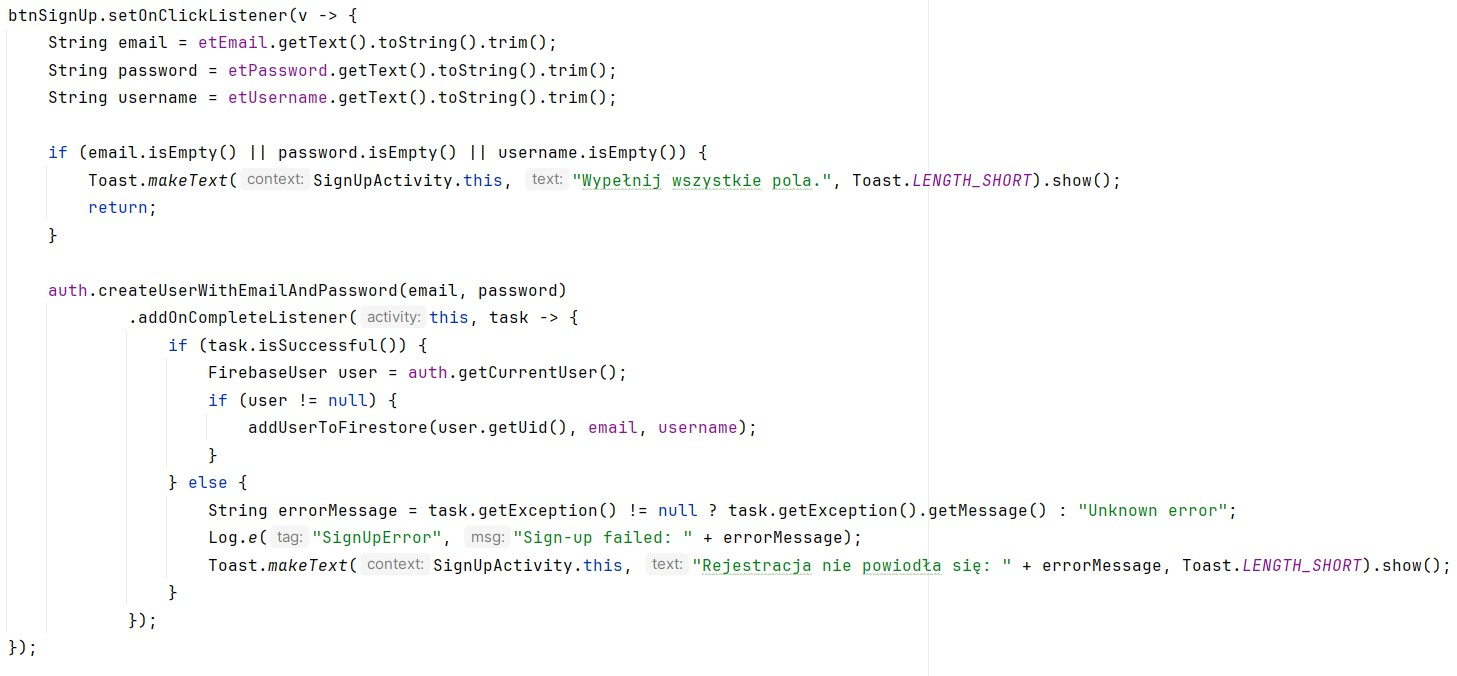
\includegraphics[width=0.6\linewidth]{img/kod/imp-reje.jpg}}
\end{minipage}
\\

Chcemy także, aby nowi użytkownicy byli zapisywani do bazy danych Firebase Firestore celem przypisania im ich aktywności na mapie. Odpowiedzialna jest za to funkcja addUserToFirestore(), która na podstawie przekazanego uid użytkownika z Firebase Authentication tworzy takiego samego użytkownika w bazie danych Firebase Firestore ze wszystkimi wprowadzonymi przez użytkownika danymi. Cała mapa z danymi zapisywana jest jako nowy dokument w bazie NoSQL, do którego można się odwołać za pomocą unikalnego uid użytkownika.\\
\noindent
\setlength{\fboxrule}{0.5pt}
\begin{minipage}{\linewidth}
    \captionof{listing}{Dodawanie użytkownika do Firebase Firestore.}
    \label{lst:addtofirestore}
    \centering
    \fbox{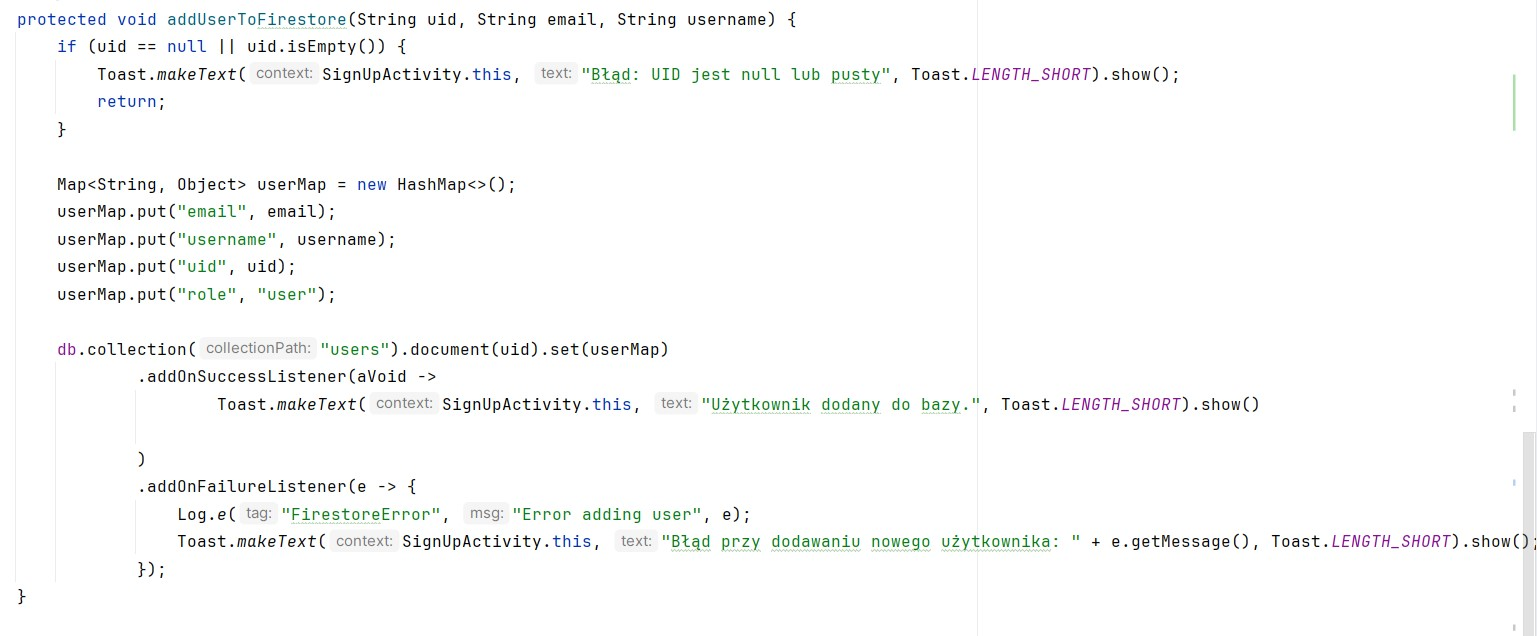
\includegraphics[width=0.6\linewidth]{img/kod/imp-addtofs.jpg}}
\end{minipage}

\noindent
\textbf{Implementacja logowania}\\
\indent Każdy użytkownik chce mieć dostęp do swoich danych, a także utworzonego konta. Logowanie pomaga nam zidentyfikować konkretnego użytkownika oraz przypisać mu jego aktywność. W tym module aplikacja również posiłkuje się Firebase Authentication. Pozwala to na szybkie logowanie użytkownika i udostępnienie mu wszystkich funkcjonalności aplikacji zgodnych z jego rolą.\\
\noindent
\setlength{\fboxrule}{0.5pt}
\begin{minipage}{\linewidth}
    \captionof{listing}{Logowanie użytkownika w "słuchaczu" przycisku "Zaloguj".}
    \label{lst:login}
    \centering
    \fbox{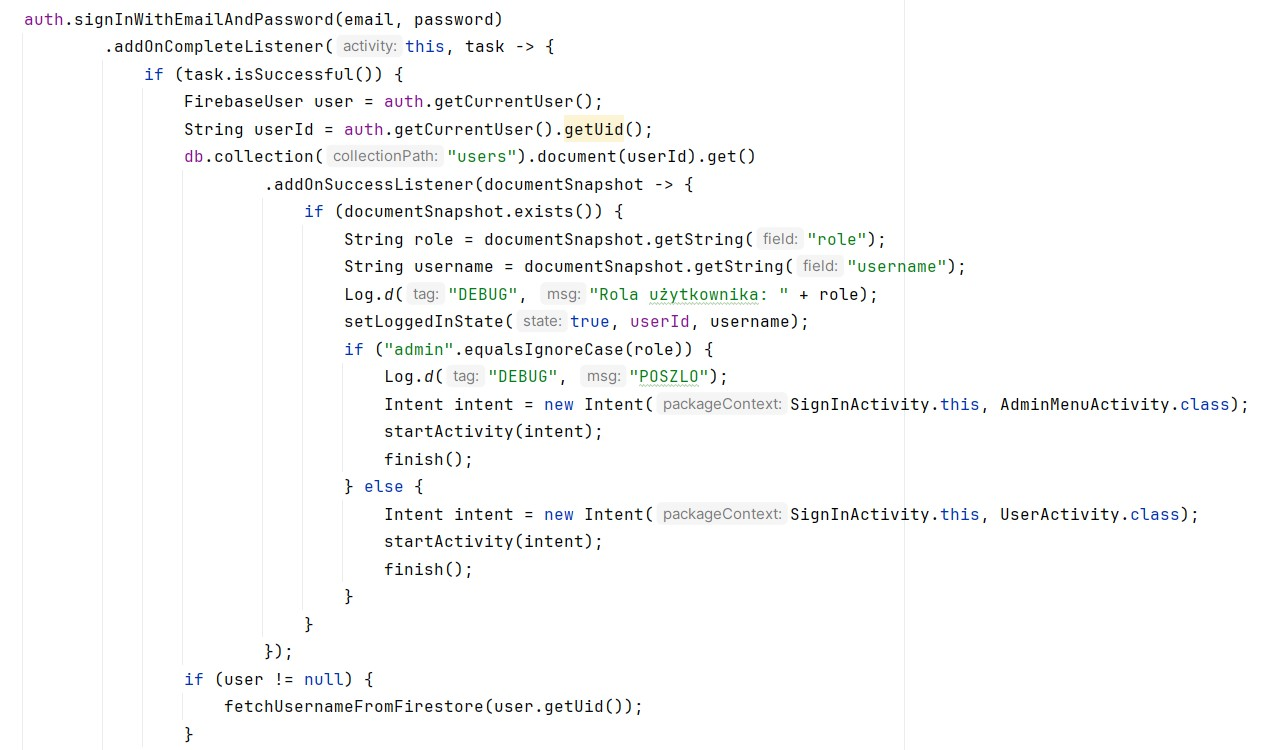
\includegraphics[width=0.6\linewidth]{img/kod/imp-login1.jpg}}
\end{minipage}


\subsection{Widoki - użytkownik}
Wygląd aplikacji został idealnie dobrany do potrzeb użytkowników, tak aby mogli bez większego problemu wykonać wszystkie akcje, które oferowane są przez system. Każdy ekran aplikacji zawiera zestaw funkcji, który umożliwia użytkownikom m.in. poruszanie się po mapie, wykonanie zgłoszenia, przejrzenie wykresu dystansów oraz wezwanie pomocy. Poniżej zostały opisane wszystkie funkcjonalności, jakie użytkownicy mogą wykonać na danym widoku aplikacji.
\\

\noindent
\textbf{Widok główny}\\
\indent Po uruchomieniu aplikacji użytkownik ma do wyboru dwie opcje “Zaloguj” oraz “Zarejestruj”, co zostało przedstawione na rys. \ref{widok:home}. Po kliknięciu danej opcji, wyświetla się formularz, który pobiera od użytkownika potrzebne dane i zapisuje je w bazie. Rejestrację przestawia rys. \ref{widok:register}, natomiast logowanie rys. \ref{widok:login}. Jeżeli użytkownik logował się już wcześniej do aplikacji, widok początkowy jest pomijany i od razu przenosi użytkownika do następnego ekranu, pokazanego na rys. \ref{widok:user}. W sytuacji, gdy zalogowanym jest administrator, wyświetlony zostanie widok aplikacji, przedstawiony na rys. \ref{widok:adminhome}. Tło na początkowym ekranie reprezentuje dwie najważniejsze funkcjonalności aplikacji t.j. wędrówki po górach oraz ostrzeganie innych o zagrożeniu. Rejestracja jest ważna, gdyż dzięki niej wiadomo kto zgłosił dane zagrożenie oraz pozwala na zbieranie danych o aktywności użytkownika.\\

\begin{figure}[H]
    \centering
    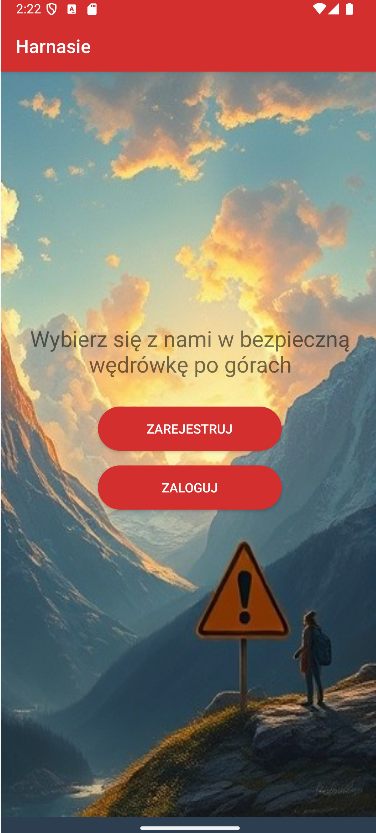
\includegraphics[scale=0.6]{img/imp/welcome.png}
    \caption{Widok początkowy po uruchomieniu aplikacji.}
    \label{widok:home}
\end{figure}

\begin{tabular}{|c|c|}
    \hline
    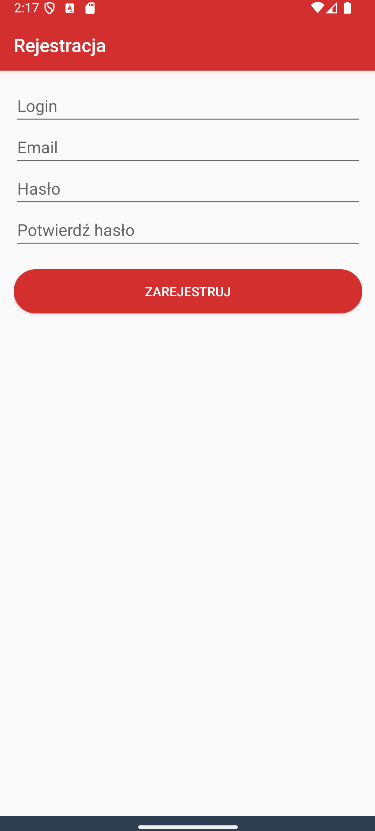
\includegraphics[width=0.4\textwidth]{img/imp/widok-reje.png} & 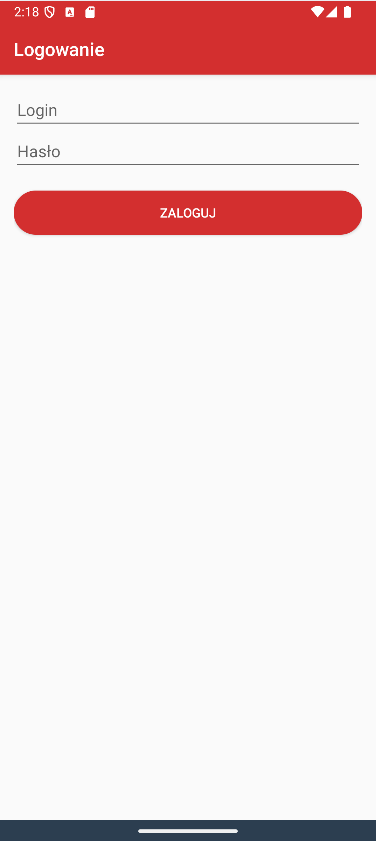
\includegraphics[width=0.4\textwidth]{img/imp/widok-log.png} \\ \hline
    \hline
    \end{tabular}

\begin{figure}[H]
    \centering
    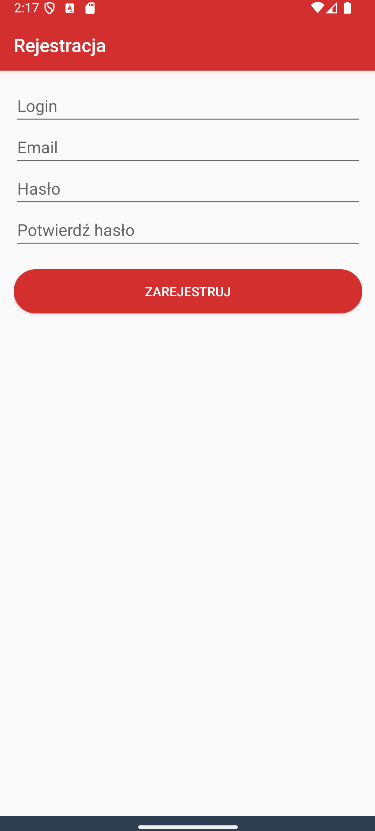
\includegraphics[scale=0.6]{img/imp/widok-reje.png}
    \caption{Widok formularza rejestracji do aplikacji.}
    \label{widok:register}
\end{figure}
\begin{figure}[H]
    \centering
    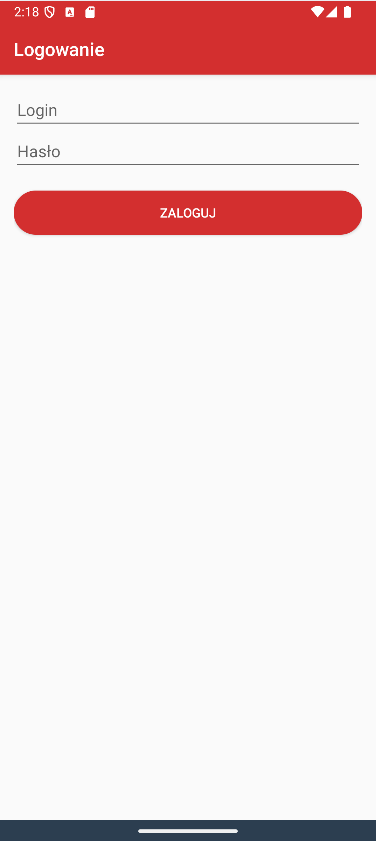
\includegraphics[scale=0.6]{img/imp/widok-log.png}
    \caption{Widok formularza logowania do aplikacji.}
    \label{widok:login}
\end{figure}
\newpage
\noindent
\textbf{Konto użytkownika} \\
\indent Na ekranie zaprezentowanym na rys.\ref{widok:user} użytkownik może zobaczyć swoją nazwę oraz wykaz pokonanych dystansów, przedstawionych w formie wykresu słupkowego. Pod nim znajduje się przycisk, dzięki któremu użytkownik może się wylogować z aplikacji. Na samym dole ekranu widoczne jest menu z czterema ikonami. Po naciśnięciu na wybrany przycisk, użytkownik zostanie przeniesiony do odpowiedniej aktywności. Pasek menu znajduje się na każdym ekranie aplikacji i umożliwia szybką nawigację między jej widokami.\\
\begin{figure}[H]
    \centering
    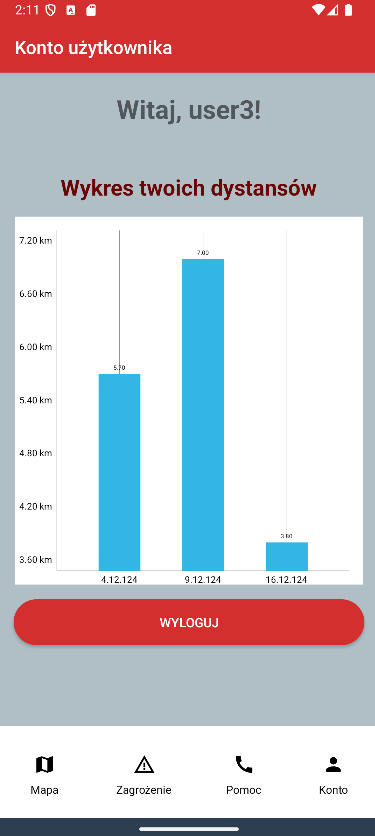
\includegraphics[scale=0.6]{img/imp/widok-user.png}
    \caption{Widok danych użytkownika z wykresem.}
    \label{widok:user}
\end{figure}

\noindent
\textbf{Widok mapy} \\
\indent Ekran mapy. przedstawiony na rys.\ref{widok:map} wyświetla szlaki Tatr oraz pozwala użytkownikowi wykonać wiele operacji m.in. zaplanować trasę oraz przejrzeć same szlaki. Wszystkie funkcjonalności będą opisane poniżej.
Ekran mapy zawiera następujące elementy:
\begin{enumerate}
    \item Ikonki ze schroniskami, szczytami oraz stawami - odpowiadają za widoczność danych markerów na mapie
    \item Ikona z warstwą - zmienia wygląd mapy z podstawowego na widoki z satelity
    \item Ikona z lokalizacją - nakierowuje mapę na obecną lokalizację użytkownika
    \item Wybierz szlak - pokazuje listę szlaków do wyboru
    \item Wyznacz trasę - umożliwia użytkownikowi podanie szczegółów trasy (początek, koniec oraz przystanki).
\end{enumerate}
Szczegółowy opis ostatnich dwóch opcji będzie przedstawiony w dalszej pracy.


\begin{figure}[H]
    \centering
    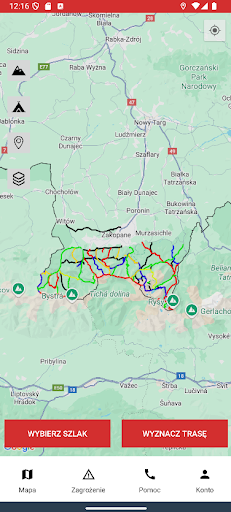
\includegraphics[scale=0.6]{img/imp/widok-mapa.png}
    \caption{Widoku mapy z narysowanymi szlakami.}
    \label{widok:map}
\end{figure}

\noindent
\textbf{Pokazywanie ikonek na mapie} \\
\indent Naciśnięcie przycisku z wybraną ikonką spododuje pojawienie się na mapie markerów w miejscu ich wystąpienia (rys. \ref{widok:ikony}). Użytkownik może kliknąć na dany znacznik w celu poznania jego nazwy oraz szczegółów w postaci informacji o wysokości n.p.m.
\noindent
\begin{figure}[H]
    \centering
    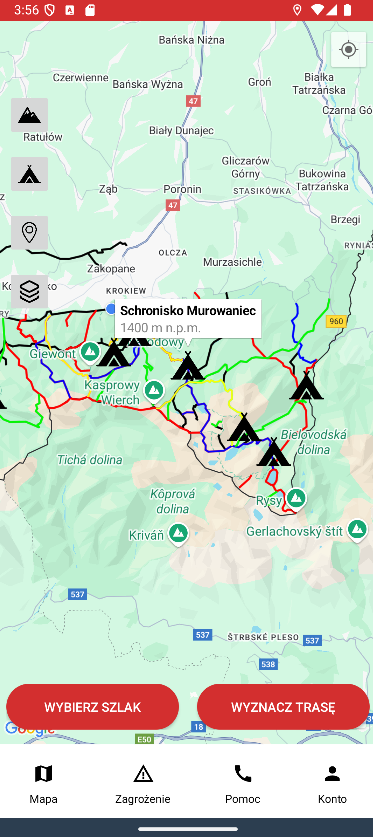
\includegraphics[scale=0.6]{img/imp/widok-ikony.png}
    \caption{Mapa z widocznymi ikonami schronisk.}
    \label{widok:ikony}
\end{figure}


\noindent
\textbf{Wyznaczanie trasy} \\
\indent Wybranie opcji “wyznacz trasę” z widoku mapy (rys. \ref{widok:wyznacztrase}) spowoduje wyświetlenie okna, które umożliwia użytkownikowi podanie szczegółów trasy. Po kliknięciu pola z punktem trasy, na środku mapy pokazuje się marker oraz przycisk do zatwierdzenia lokalizacji, co zostało przedstawione na rys.\ref{widok:ustawlokalizacje} Potwierdzenie wybranej lokalizacji spowoduje, iż w miejscu pola z punktem trasy pojawia się jej nazwa (rys. \ref{widok:ustawlokalizacjewynik}). Użytkownik w każdej chwili może zmienić ustawione punkty trasy, ponownie klikając w wybrane pole. W przypadku włączonej lokalizacji, pole z początkiem trasy jest uzupełnione już o współrzędne wędrówkowicza. Po ustawieniu wszystkich pól z punktami trasy, użytkownik może wybrać następujące opcje:
\begin{itemize}
    \item Dodaj przystanek - pokazuje pole do podania jego lokalizacji,
    \item Zatwierdź - wyznacza na mapie trasę, którą stworzył użytkownik po podaniu wszystkich potrzebnych punktów,
    \item Usuń - usuwa przystanek z trasy
\end{itemize}

\begin{figure}[H]
    \centering
    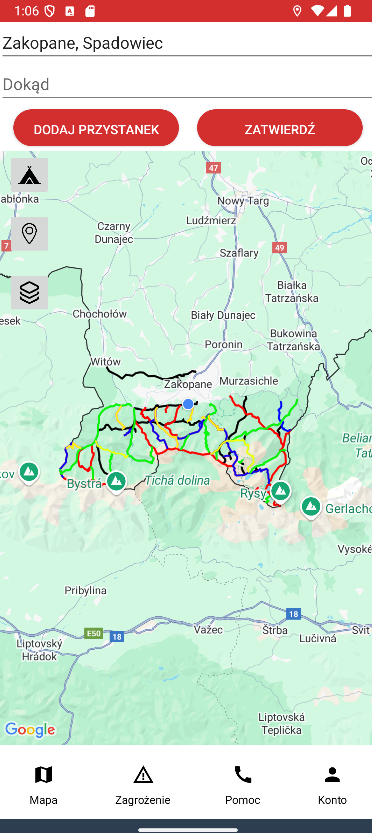
\includegraphics[scale=0.6]{img/imp/widok-loka.png}
    \caption{Opcje widoczne po kliknięciu przycisku "Wyznacz trasę".}
    \label{widok:wyznacztrase}
\end{figure}

\begin{figure}[H]
    \centering
    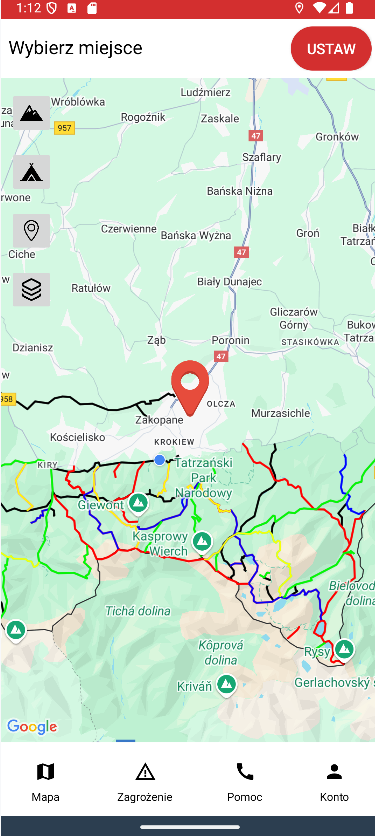
\includegraphics[scale=0.6]{img/imp/widok-marker.png}
    \caption{Wybór punktów trasy za pomocą markera.}
    \label{widok:ustawlokalizacje}
\end{figure}


\begin{figure}[H]
    \centering
    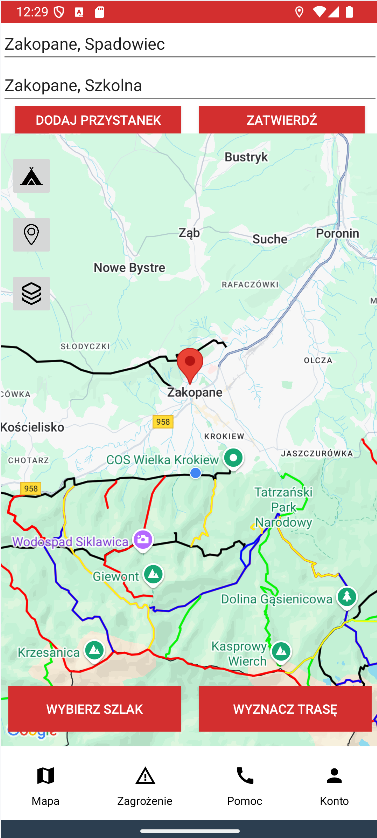
\includegraphics[scale=0.6]{img/imp/widok-pkt.png}
    \caption{Rezultat wyboru lokalizacji punktu trasy.}
    \label{widok:ustawlokalizacjewynik}
\end{figure}

\noindent
\textbf{Zatwierdzanie trasy} \\
\indent Po zatwierdzeniu trasy, pokazuje się ona na mapie wraz z kolejnych opcjami, które zostały przedstawione na rys. \ref{widok:zatwierdztrase}:
\begin{itemize}
    \item Usuń trasę - powoduje usunięcie trasy oraz markerów oznaczających kolejne jej punkty,
    \item Google - umożliwia użytkownikowi na nawigację po szlaku za pomocą aplikacji Mapy Google.\\
\end{itemize}

\begin{figure}[H]
    \centering
    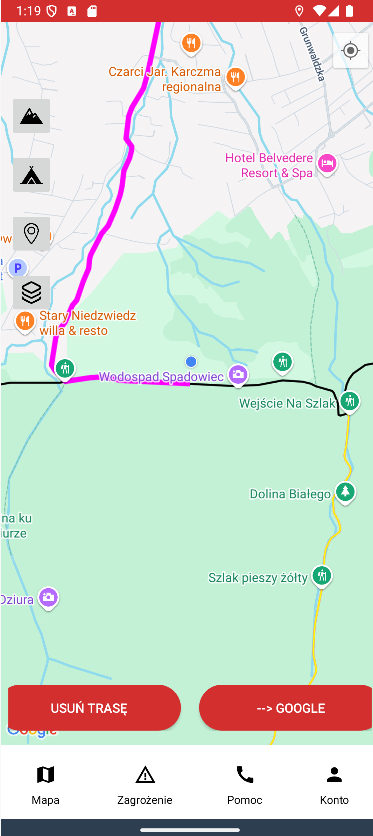
\includegraphics[scale=0.6]{img/imp/widok-trasa.png}
    \caption{Widok aplikacji po zatwierdzeniu wybranej przez użytkownika trasy.}
    \label{widok:zatwierdztrase}
\end{figure}

\noindent
\textbf{Wybieranie szlaku} \\
\indent Po wybraniu opcji “Wybierz szlak” z widoku mapy (rys. \ref{widok:map}) pokaże się lista szlaków \\z oznaczeniem koloru, widoczna na rys. \ref{widok:wyborszlaku}. Użytkownik może przeszukać wszystkie szlaki górskie Tatr, a po kliknięciu przycisku “wybierz”, zostaje nakierowany na początek wybranej trasy, jak zostało przedstawione na rys. \ref{widok:szlak}. Na ekranie widoczna jest także kolejna opcja, która umożliwia użytkownikowi nawigację po trasie za pomocą aplikacji Mapy Google.\\

\begin{figure}[H]
    \centering
    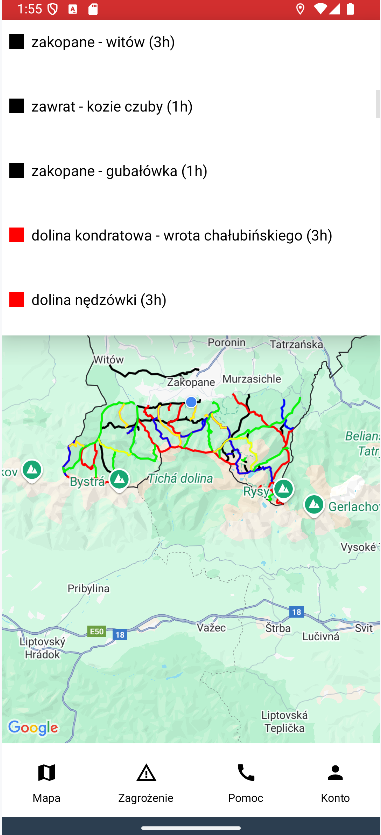
\includegraphics[scale=0.6]{img/imp/lista_szlakow.png}
    \caption{Lista dostępnych szlaków.}
    \label{widok:wyborszlaku}
\end{figure}

\begin{figure}[H]
    \centering
    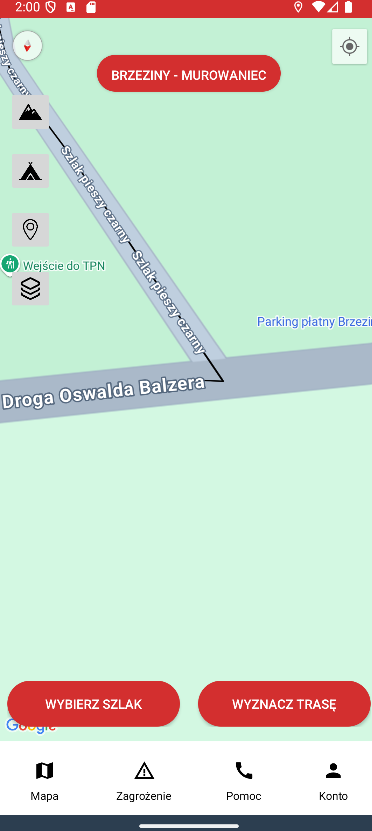
\includegraphics[scale=0.6]{img/imp/po-wyborze-z-listy.png}
    \caption{Widok z początkiem wybranego z listy szlaku.}
    \label{widok:szlak}
\end{figure}
\newpage
\noindent
\textbf{Widok formularza zgłoszeń zagrożeń} \\
\indent Ekran zgłoszenia pokazany na rys. \ref{widok:zgłoszenie} spełnia jedno z podstawowych funkcjonalności aplikacji. To tutaj użytkownik, mając włączoną lokalizację i internet, może wygenerować powiadomienie dla innych użytkowników o danym zagrożeniu na szlaku, wybierając jego typ z listy i opisując szczegóły. Po naciśnięciu “Zgłoś zagrożenie”, zgłoszenie zostaje od razu wysłane lub w przypadku problemów z internetem, zapisane i wysłane natychmiast po ponownym nawiązaniu połączenia.

\begin{figure}[H]
    \centering
    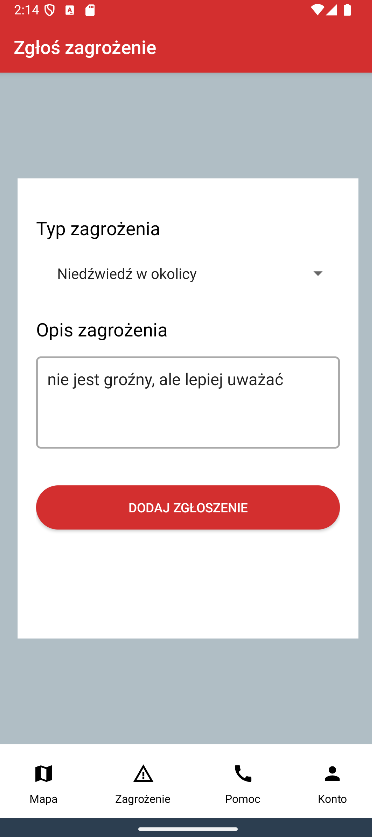
\includegraphics[scale=0.70]{img/imp/widok-danger.png}
    \caption{Widok z formularzem zgłoszeniowym dla zagrożeń.}
    \label{widok:zgłoszenie}
\end{figure}

\noindent
\textbf{Widok ekranu z numerami alarmowymi} \\
\indent Ekran aplikacji, pokazany na rys. \ref{widok:telefony} umożliwia użytkownikowi wezwanie pomocy \\w razie wypadku. Kliknięcie przycisków po lewej stronie spowoduje zadzwonienie na dany numer, natomiast przyciski po prawej pozwalają na skopiowanie numeru telefonu. Jest to bardzo wygodna opcja, która oszczędza użytkownikowi dużo czasu, gdyż nie musi go szukać i ma zawsze pod ręką.

\begin{figure}[H]
    \centering
    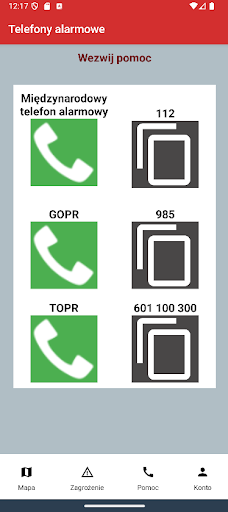
\includegraphics[scale=0.6]{img/imp/widok-telefony.png}
    \caption{Widok ekranu z numerami alarmowymi.}
    \label{widok:telefony}
\end{figure}

\subsection{Widoki - administrator}
Dodając do dowolnego zarejestrowanego użytkownika rolę administratora, zmieni się zupełnie wygląd jego aplikacji po zalogowaniu. Administrator ma dostęp do kompletnie innych funkcjonalności niż zwykły użytkownik. Należą do nich: dodawanie nowych szlaków do Firebase Storage w formacie .kml oraz akceptowanie zgłoszeń o zagrożeniach przesłanych przez użytkowników. Poniżej znajduje się pełny opis wyglądu i funkcjonalności aplikacji użytkownika z rolą "administrator".
\\

\noindent
\textbf{Widok główny administratora}\\
\indent Administrator posiada swoją własną wersję aplikacji. Jego ekran główny \ref{widok:adminhome} posiada zestaw przycisków odpowiedzialnych za główne elementy, którymi zarządza. Kolejno od góry widoczne są przyciski "Wyślij powiadomienie ogólne", przenoszący go do widoku krótkiego formularza (rys. \ref{widok:admindanger}), gdzie może wkleić treść komunikatu od służb tatrzańskich lub napisać własną treść powiadomienia wysyłanego do wszystkich użytkowników, "Pokaż wszystkie zgłoszenia" przenoszący do widoku listy wszystkich zgłoszonych zagrożeń (rys. \ref{widok:adminaccept}) czekających na akceptację, "Dodaj trasę" przenoszący do widoku umożliwiającego dodanie nowego szlaku do bazy (rys. \ref{widok:kml}) oraz "Wyloguj" zamykający bieżącą sesję użytkownika.
\begin{figure}[H]
    \centering
    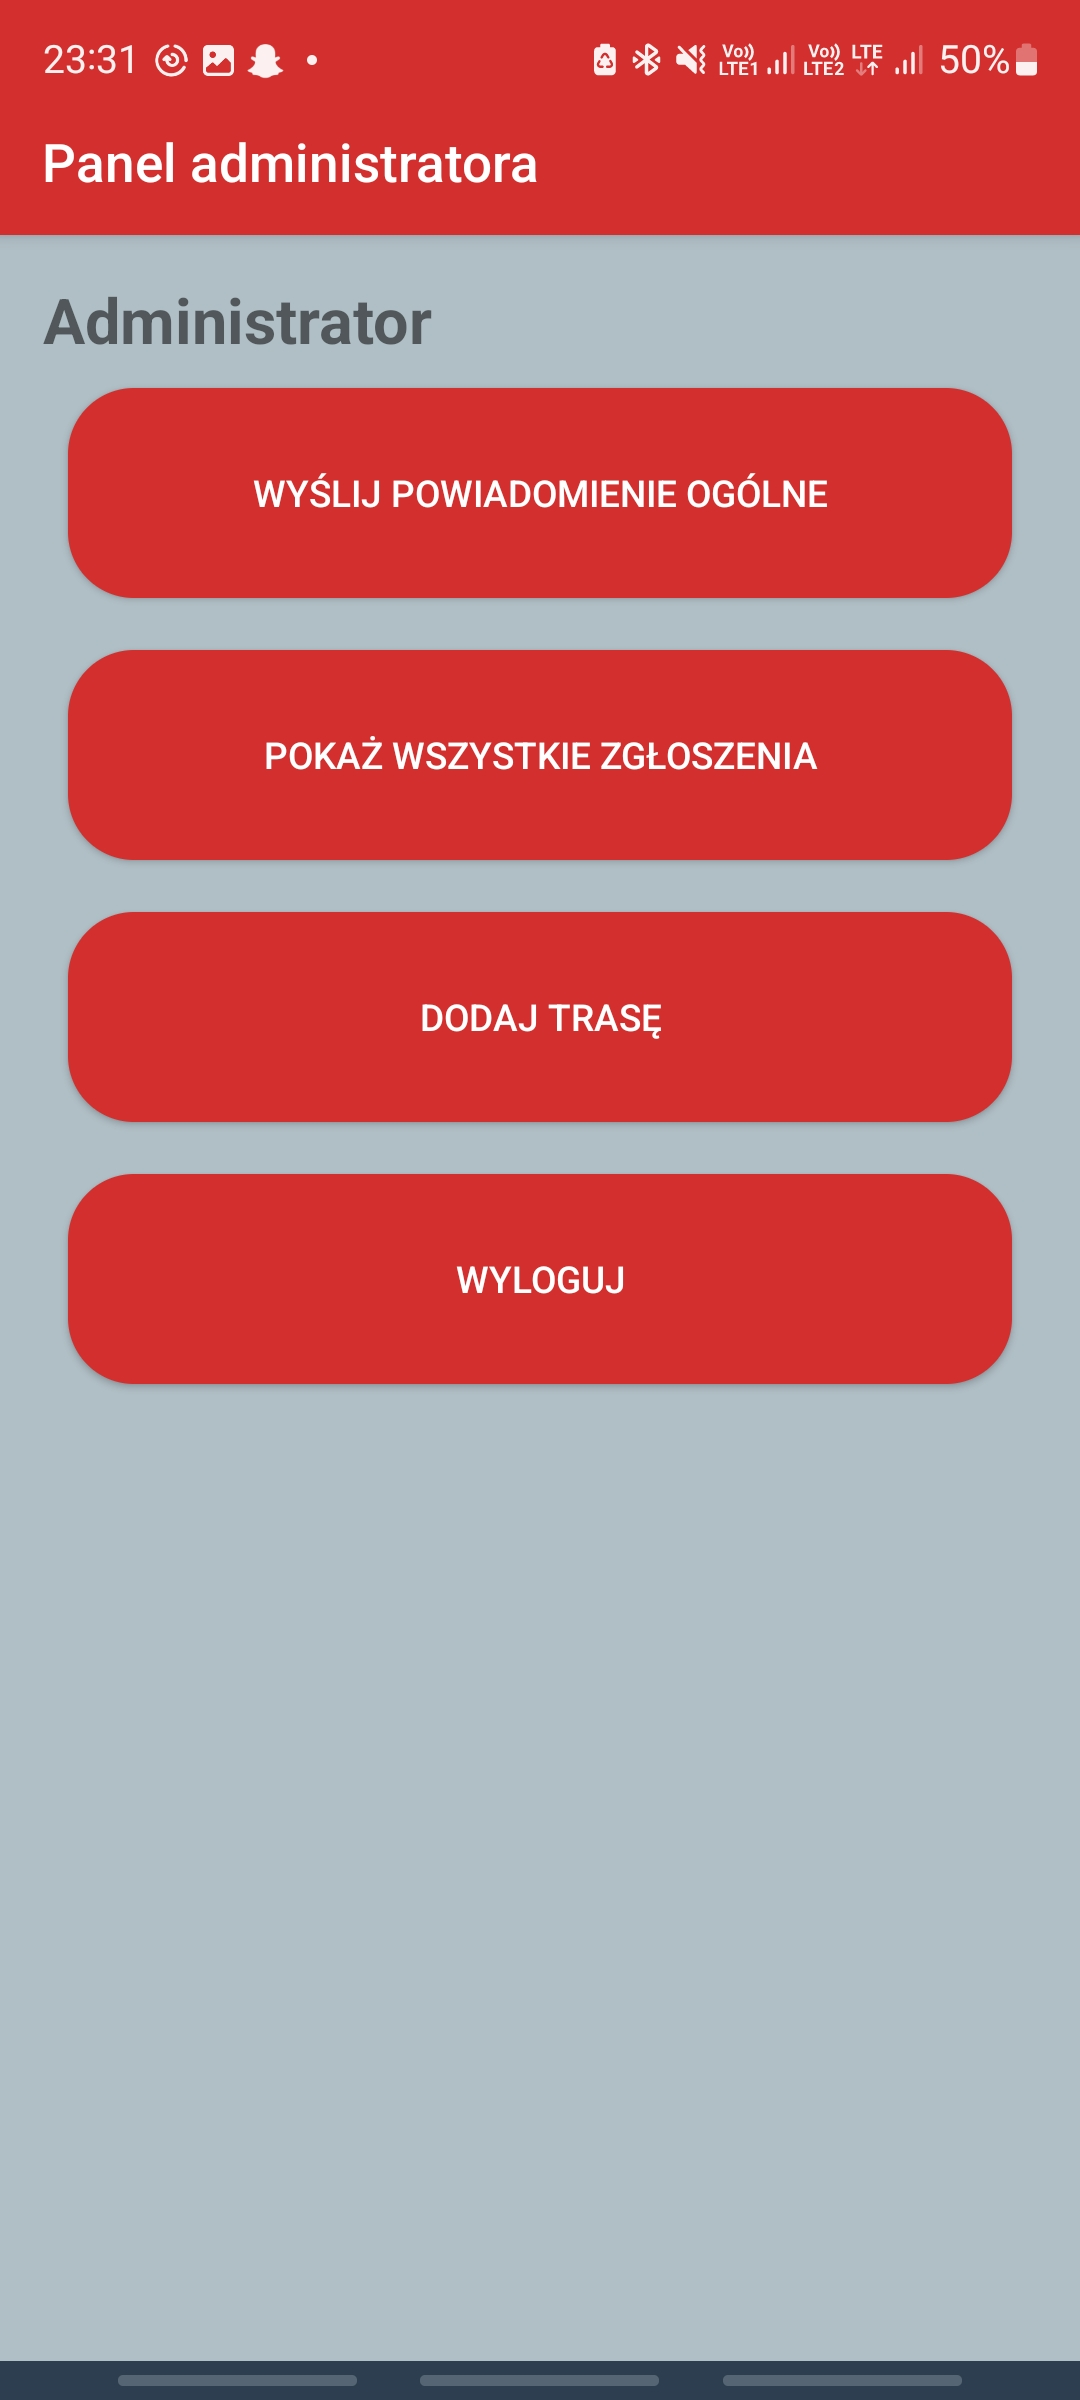
\includegraphics[scale=0.15]{img/imp/widok-admin-home.jpg}
    \caption{Widok główny po zalogowaniu na konto z uprawnieniami administratora.}
    \label{widok:adminhome}
\end{figure}

\noindent
\textbf{Widok formularza komunikatów}\\
\indent Formularz przedstawiony na poniższym widoku (rys. \ref{widok:admindanger}) umożliwia administratorowi wysłanie powiadomień do wszystkich użytkowników jednocześnie z komunikatami bezpieczeństwa wydawanymi przez TOPR, GOPR lub TPN najczęściej dotyczących stanu meteorologicznego panującego w Tatrach.
\begin{figure}[H]
    \centering
    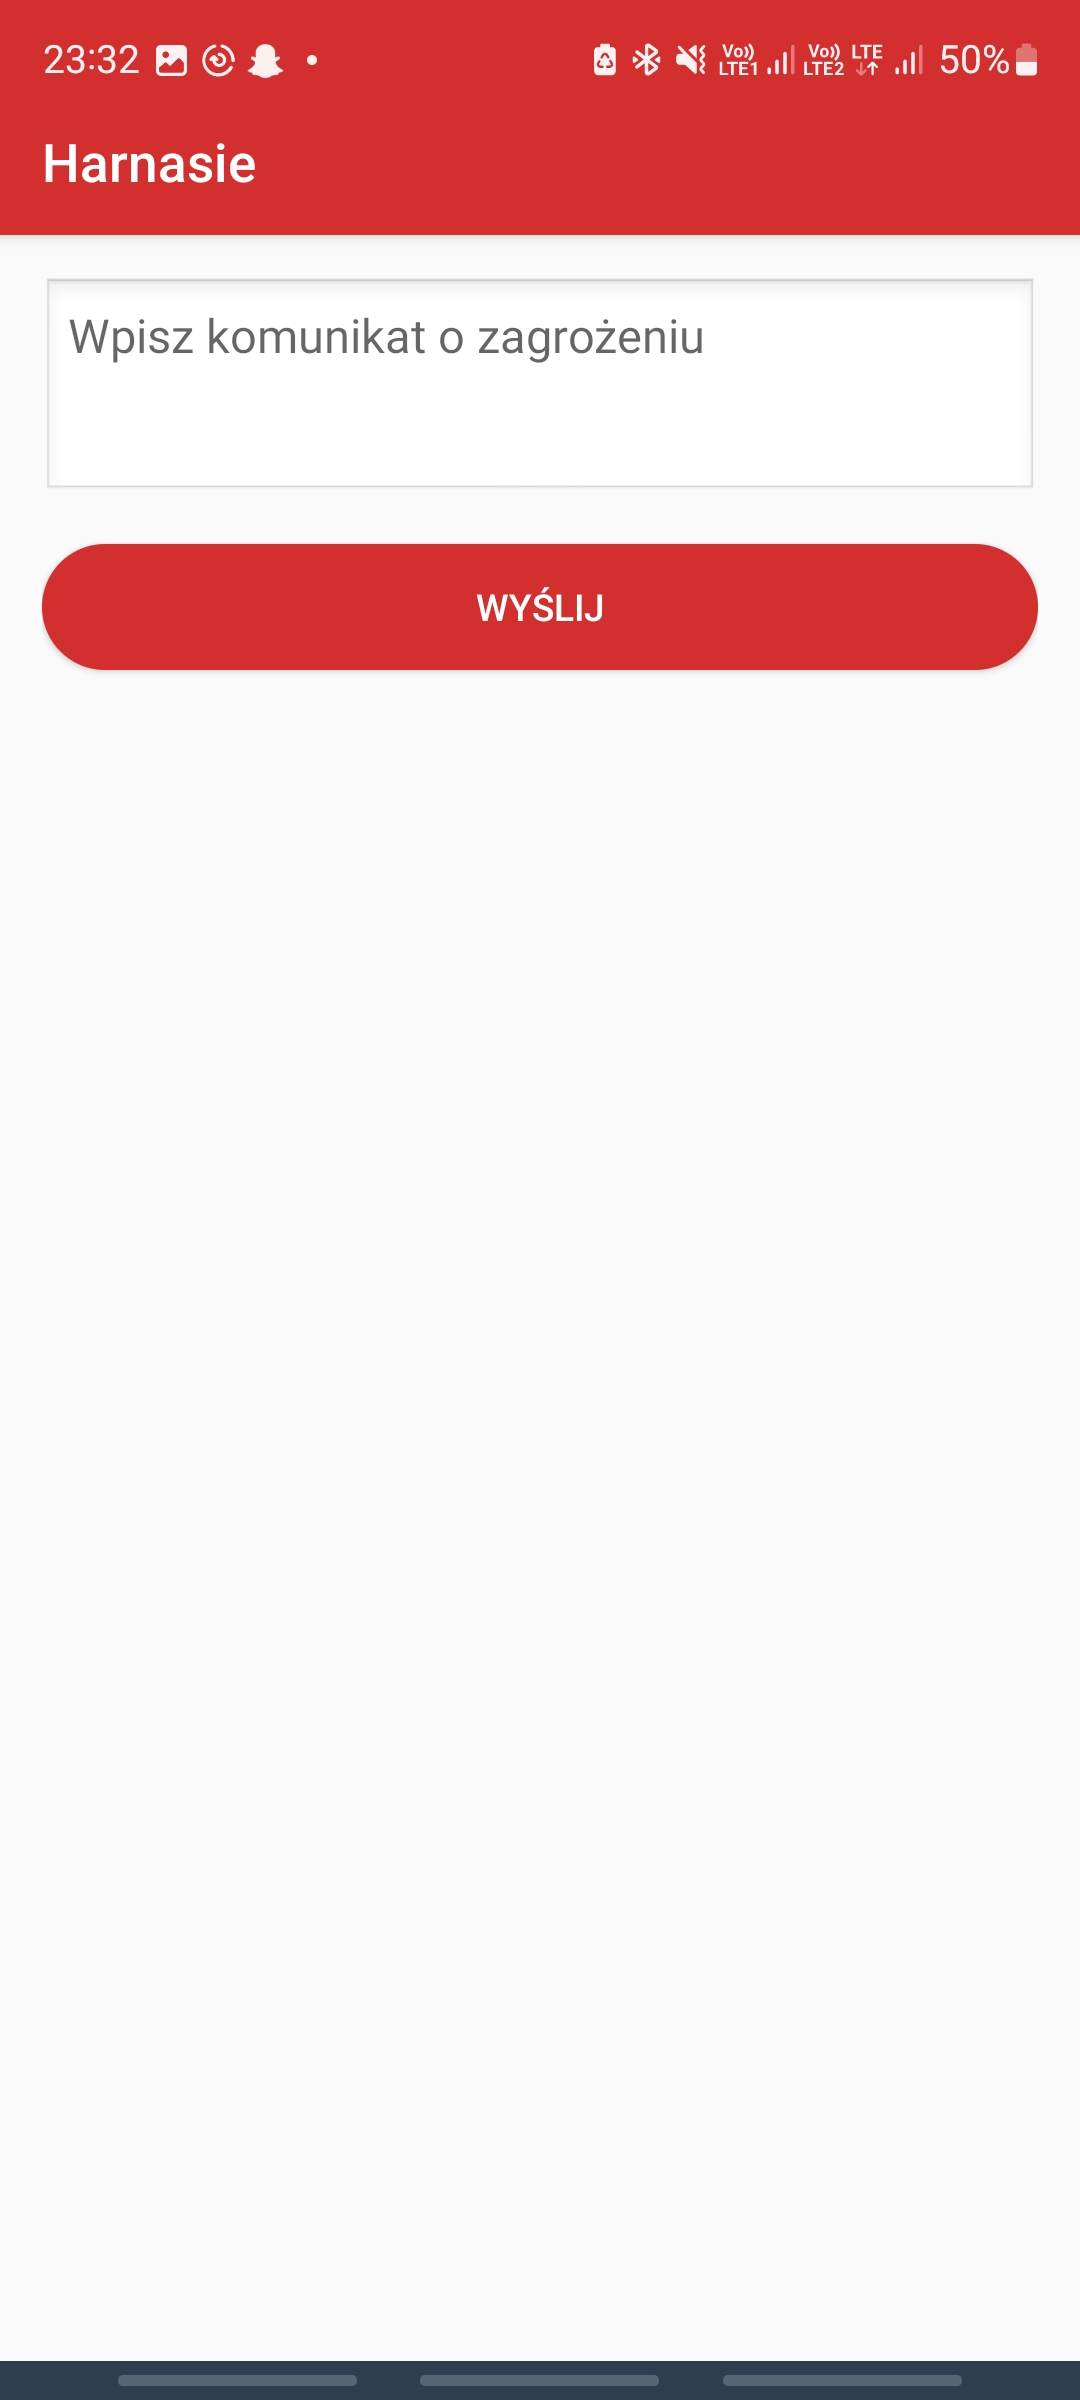
\includegraphics[scale=0.15]{img/imp/widok-admin-danger.jpg}
    \caption{Widok formularza administratora do przekazywania komunikatów TOPR, GOPR, TPN w formie powiadomienia dla wszystkich użytkowników.}
    \label{widok:admindanger}
\end{figure}

\noindent
\textbf{Widok listy zgłoszeń}\\
\indent Poniższy widok (rys. \ref{widok:adminaccept}) przedstawia listę zgłoszonych przez użytkowników zagrożeń na trasie, które czekają na akceptację po stronie administratora. Każde zgłoszenie musi mieć swój typ oraz krótki opis, a aplikacja zbiera dodatkowo informacje o aktualnym miejscu użytkownika w momencie wysłania zgłoszenia (nawet offline) oraz jego identyfikator.
\begin{figure}[H]
    \centering
    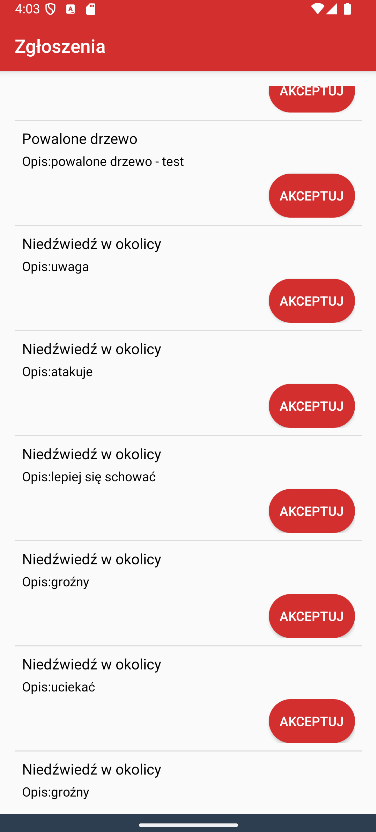
\includegraphics[scale=0.6]{img/test/testdanger.png}
    \caption{Widok administratora z listą zagrożeń do zaakceptowania.}
    \label{widok:adminaccept}
\end{figure}

\noindent
\textbf{Widok wspomagający dodawanie szlaków do bazy} \\ 
\indent Poniższy widok (rys. \ref{widok:kml}) przedstawia prosty proces dodawania plików .kml z nowymi szlakami. Najpierw administrator wyznacza przebieg szlaku za pomocą strony Google My Maps, gdzie ma możliwość eksportowania pliku z nowo utworzonym szlakiem do formatu .kml. Następnie może wybrać świeżo przygotowany plik i spróbować wysłać go do usługi Firebase Storage. Pojawia się jednak jeden problem - w procesie implementacji tej funkcji oraz testowania jej poprawnego działania okazało się, że urządzenia mobilne mogą zapisywać pliki .kml jako pliki .xml. Dlatego zdecydowano się na dodanie kolejnego przycisku "Otwórz konwerter xml na kml", który przenosi administratora na przeglądarkowy konwerter plików. Wyeksportowany, przekonwertowany plik administrator wysyła na serwer za pomocą przycisku "Prześlij plik".
\begin{figure}[H]
    \centering
    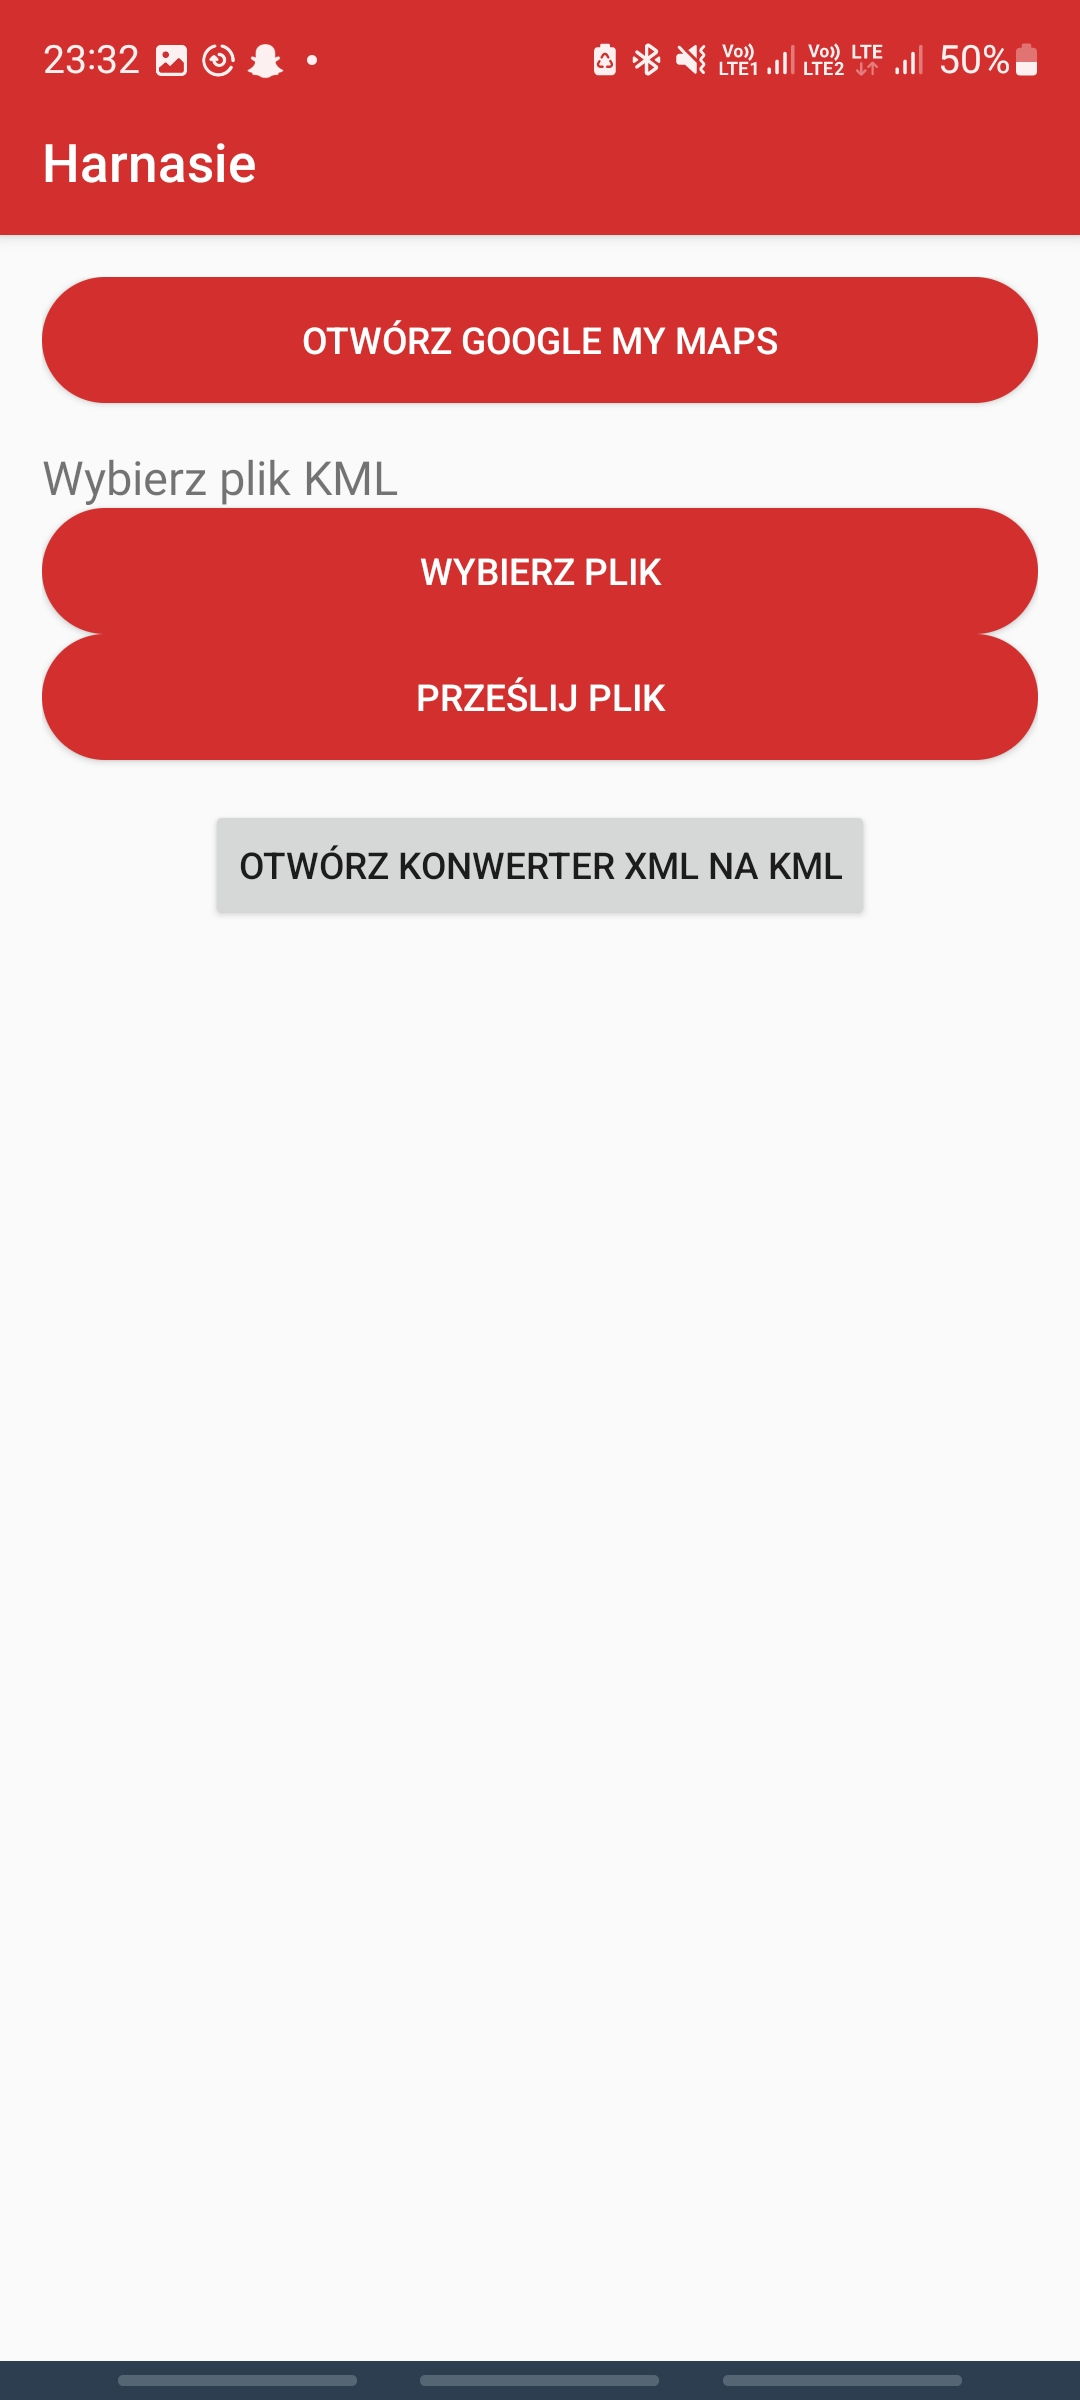
\includegraphics[scale=0.15]{img/imp/widok-dodajkml.jpg}
    \caption{Widok administratora z przeprowadzeniem krok po kroku po procedurze dodania nowych szlaków do bazy dostępnych szlaków.}
    \label{widok:kml}
\end{figure}







